\chapter{Ancestors and Descendants}
\label{chap:ancestor}
In this Chapter you will:
\begin{enumerate}
\item Use sub-properties and the transitive property characteristic to infer ancestors of people;
\item Add properties to the \fhkb property hierarchy that will infer ancestors and descendants of a person without adding any more facts to the \fhkb;
\item Explore the use of sub-property chains for grandparents, great grandparents and so on;
\item Place all of these new object properties in the property hierarchy and in that way learn more about the implications of the property hierarchy.
\end{enumerate}

\snapshot{Find a snapshot of the ontology at this stage at \fhkbhome.}

\section{Ancestors and Descendants}

The \fhkb has parents established between individuals and we know that all people have two parents. A parent is an ancestor of its children; a person's parent's parents are its ancestors; and so on. So, in our \fhkb, Robert's ancestors are David, Margaret, William, Iris, Charles, Violet, James, another Violet, another William, Sarah and so on. If my parent's parents are my ancestors, then what we need is a transitive version of the \con{hasParent} property. Obviously we do not want \con{hasParent} to be transitive, as Robert's grandparents (and so on) would become his parents (and that would be wrong).

We can easily achieve what is necessary. We need a \con{hasAncestor} property that has a transitive characteristic. The trick is to make this a super-property of the \con{hasParent} property. As explained before, a sub-property implies its super-property. So, if \indiv \emph{x} holds a \con{hasParent} property with an \indiv \emph{y}, then it also holds an instance of its super-property \con{hasAncestor} with the \indiv \emph{y}. If \indiv \emph{y} then holds a \con{hasParent} property with another \indiv \emph{z}, then there is also, by implication, a \con{hasAncestor} property between \emph{y} and \emph{z}. As \con{hasAncestor} is transitive, \emph{x} and \emph{z} also hold a \con{hasAncestor} relationship between them.

The inverse of \con{hasAncestor} can either be \con{isAncestorOf} or \con{hasDescendant}. We choose the \con{isAncestorOf} option.

\steps{Object properties: exploiting the semantics}{
\item Make a new object property \con{hasRelation}, make it symmetric.
\item Make a new object property \con{hasAncestor}.
\item Make it a sub-property of \con{hasRelation} and a super-property of \con{hasParent}.
\item Make \con{hasAncestor} transitive.
\item Create the inverse \con{isAncestorOf}. Do not `stitch' it into the property hierarchy; the reasoner will sort it all out for you.
\item Run the reasoner and issue the DL query \con{hasAncestor value \iwgs}.
\item Issue the query \con{isAncestorOf value \irds}.
}

The \con{hasAncestor} object property will look like this:

\owlcode{
ObjectProperty: hasAncestor

    SubPropertyOf: 
        hasRelation

    SuperPropertyOf: 
        hasParent,

    Characteristics: 
        Transitive

    InverseOf: 
        isAncestorOf
}\\\\
As usual, it is best to think of the objects or individuals involved in the relationships. Consider the three individuals -- Robert, David and William. Each has a \con{hasFather} property, linking Robert to David and then David to William. As \con{hasFather} implies its super-property \con{hasParent}, Robert also has a \con{hasParent} property with David, and David has a \con{hasParent} relation to William. Similarly, as \con{hasParent} implies \con{hasAncestor}, the Robert object has a \con{hasAncestor} relation to the David object and the David object has one to the William object. As \con{hasAncestor} is transitive, Robert not only holds this property to the David object, but also to the William object (and so on back through Robert's ancestors).

\section{Grandparents and Great Grandparents}

We also want to use a sort of restricted transitivity in order to infer grandparents, great grandparents and so on. My grandparents are my parent's parents; my grandfathers are my parent's fathers. My great grandparents are my parent's parent's parents. My great grandmothers are my parent's parent's mothers. This is sort of like transitivity, but we want to make the paths only a certain length and, in the case of grandfathers, we want to move along two relationships -- \con{hasParent} and then \con{hasFather}.

We can do this with \owlii's sub-property chains. The way to think about sub-property chains is: If we see property \emph{x} followed by property \emph{y} linking three objects, then it implies that property \emph{z} is held between the first and third objects. Figure~\ref{fig:chain_triangle} shows this diagrammatically for the hasGrandfather property.

\begin{figure}
\begin{center}
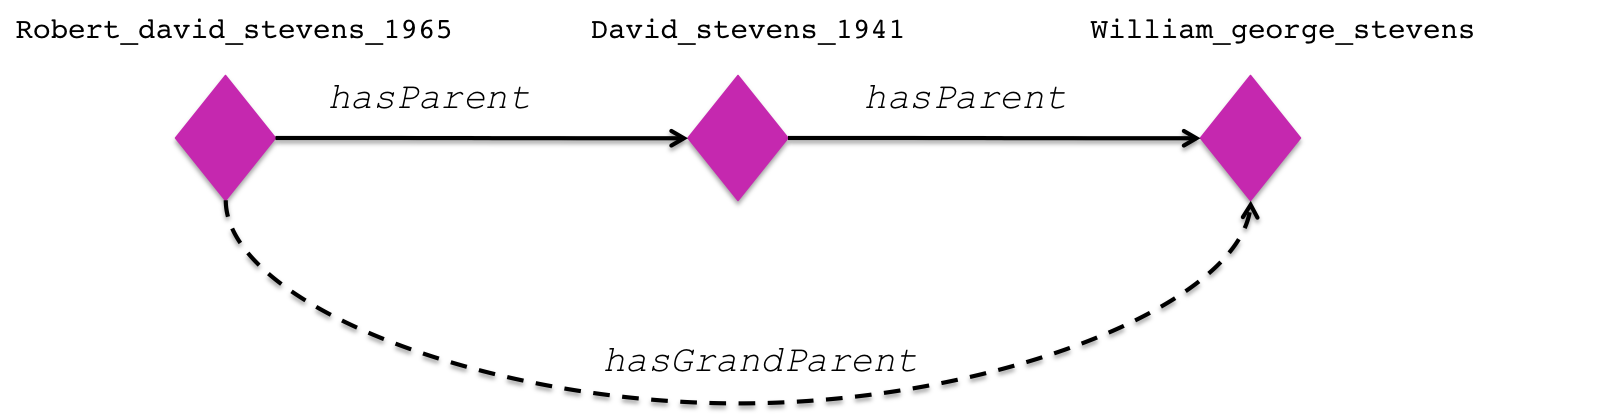
\includegraphics[width=\figwidth]{figures/grandparent}\caption{Three blobs representing objects of the class \person. The three objects are linked by a \con{hasParent} property and this implies a \con{hasGrandparent} property.}\label{fig:chain_triangle}
\end{center}
\end{figure}

For various grandparent object properties we need the following sets of implications:
\begin{itemize}
\item My parent's parents are my grandparents;
\item My parent's fathers are my grandfathers;
\item My parent's mothers are my grandmothers;
\item My parent's parent's parents are my great grandparents or my grandparent's parents are my great grandparents.
\item My parent's parent's fathers are my great grandfathers or my parent's grandfathers are my great grandfathers;
\item My parent's parent's mothers are my great grandmothers (and so on).
\end{itemize}

Notice that we can trace the paths in several ways, some have more steps than others, though the shorter paths themselves employ paths. Tracing these paths is what \owlii's sub-property chains achieve. For the new object property \con{hasGrandparent} we write:
\\\\
\owlcode{
ObjectProperty: hasGrandparent
SubPropertyChain:
hasParent o hasParent
}
\\\\
We read this as `\con{hasParent} followed by \con{hasParent} implies \con{hasGrandparent}'.
We also need to think where the \con{hasGrandparent} property fits in our growing hierarchy of object properties. Think about the implications: Does holding a \con{hasParent} property between two objects imply that they also hold a \con{hasGrandparent} property? Of course the answer is `no'. So, this new property is not a super-property of \con{hasParent}. Does the holding of a \con{hasGrandparent} property between two objects imply that they also hold an \con{hasAncestor} property? The answer is `yes'; so that should be a super-property of \con{hasGrandparent}. We need to ask such questions of our existing properties to work out where we put it in the object property hierarchy. At the moment, our \con{hasGrandparent} property will look like this:
\\\\
\owlcode{
ObjectProperty: hasGrandParent

    SubPropertyOf: 
        hasAncestor
    
    SubPropertyChain:
		hasParent o hasParent

    SuperPropertyOf: 
        hasGrandmother,
        hasGrandfather


    InverseOf: 
        isGrandParentOf
}
\\
Do the following task:
\steps{Grandparents object properties}{
\item Make the \con{hasGrandparent}, \con{hasGrandmother} and \con{hasGrandfather} object properties and the obvious inverses (see OWL code above);
\item Go to the individuals tabs and inspects the inferred object property assertions for \irds and his parents.
}

Again, think of the objects involved. We can take the same three objects as before: Robert, David and William. Think about the properties that exist, both by assertion and implication, between these objects. We have asserted only \con{hasFather} between these objects. The inverse can be inferred between the actual individuals (remember that this is not the case for class level restrictions -- that all instances of a class hold a property does not mean that the filler objects at the other end hold the inverse; the quantification on the restriction tells us this). Remember that:
\begin{enumerate}
\item Robert holds a \con{hasFather} property with David;
\item David holds a \con{hasFather} property with William;
\item By implication through the \con{hasParent} super-property of \con{hasFather}, Robert holds a \con{hasParent} property with David, and the latter holds one with William;
\item The sub-property chain on \con{hasGrandfather} then implies that Robert holds a \con{hasGrandfather} property to William. Use the diagram in figure~\ref{fig:chain_triangle} to trace the path; there is a \con{hasParent} path from Robert to William via David and this implies the \con{hasGrandfather} property between Robert and William.
\end{enumerate}

It is also useful to point out that the inverse of \con{hasGrandfather} also has the implication of the sub-property chain of the inverses of \con{hasParent}. That is, three objects linked by a path of two \con{isParentOf} properties implies that an \con{isGrandfatherOf} property is established between the first and third object, in this case William and Robert. As the inverses of \con{hasFather} are established by the reasoner, all the inverse implications also hold.

\section{Summary}

It is important when dealing with property hierarchies to think in terms of properties between objects and of the implications `up the hierarchy'. A sub-property implies its super-property. So, in our \fhkb, two person objects holding a \con{hasParent} property between them, by implication also hold an \con{hasAncestor} property between them. In turn, \con{hasAncestor} has a super-property \con{hasRelation} and the two objects in question also hold, by implication, this property between them as well.

We made \con{hasAncestor} transitive. This means that my ancestor's ancestors are also my ancestors. That a sub-property is transitive does not imply that its super-property is transitive. We have seen that by manipulating the property hierarchy we can generate a lot of inferences without adding any more facts to the individuals in the \fhkb. This will be a feature of the whole process -- keep the work to the minimum (well, almost).

In \owlii, we can also trace `paths' around objects. Again, think of the objects involved in the path of properties that link objects together. We have done simple paths so far -- Robert linked to David via \con{hasParent} and David linked to William via \con{hasFather} implies the link between Robert and William of \con{hasGrandfather}. If this is true for all cases (for which you have to use your domain knowledge), one can capture this implication in the property hierarchy. Again, we are making our work easier by adding no new explicit facts, but making use of the implication that the reasoner works out for us.

\expressivity{ALRI+}

\ctime{262}{30}{4}